\documentclass[12pt]{article}
\usepackage[a4paper,left=27mm,right=27mm,top=24mm,bottom=22mm]{geometry}
\usepackage[space]{ctex}
\usepackage{graphicx}
\usepackage{float}
\usepackage{subfigure}
\usepackage{amsmath}
\usepackage{amsfonts,amssymb}
\title{\LARGE\textbf{ImageWarping}}
\author{SA21010060 周俊亦}
\date{}

\begin{document}
	\maketitle
	\renewcommand{\abstractname}{Abstract}
	\begin{abstract}
		图像变形是插值算法的重要应用之一。本报告复现了两种经典的插值算法: IDW(Inverse distance-weighted)和 RBF(Radial basis functions).
	\end{abstract}
	
	\section{算法原理}
		\subsection{概述}
		将图像看成二次函数,就像在三维平面上波澜起伏的山峰一般,可以对图像进行非常有趣的操作,例如图像变形就是应用之一。借助傅里叶变换\footnote{写作业时的胡思乱想:傅里叶变换真是神奇而又伟大的变换。万物皆可分解,万物本就同源。旋转的sin和cos,就像精密的齿轮啮合,滚动走出正弦轨迹,再复杂的事物,都逃不过拟合,看似复杂的命运,背后是不是也有一根牵引的线呢?}的思想,通过离散点拟合,可以将图像分解成一系列基函数(其中高斯基函数理论上可以拟合任意复杂的函数)。通过这些基函数,我们可以利用插值算法将图像重新“塑形”。
		
		
		
		\begin{figure}[H]
			\centering
			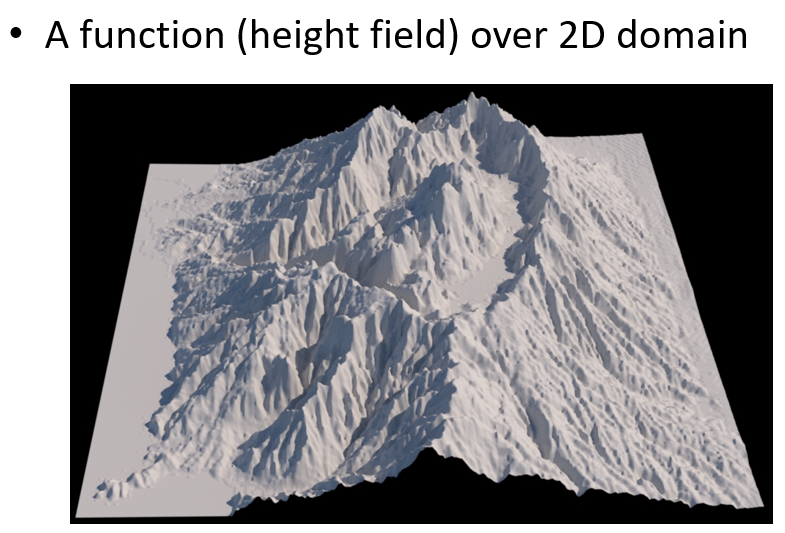
\includegraphics[width=3.3in]{./ppt1.png}
			\centering
			\caption{另一角度的灰度图}
		\end{figure}
	
		\subsection{原理}
		算法的输入输出描述为:\\
		\textbf{Input}: 给定$n$对控制点对$(\textbf{p}_i,\textbf{q}_i)$,其中
		$\textbf{p}_i(x_{p_i},y_{p_i}),\textbf{q}_i(x_{q_i},y_{q_i}),\textbf{p}_i,\textbf{q}_i\in \mathbb{R}^{2}, i=1,2, \cdots, n$.\\
		\textbf{Output}:\space(An at-least-continues function)\space$\mathbf{f}: \mathbb{R}^{2} \rightarrow \mathbb{R}^{2}, \text {使得} \,\mathbf{f}\left(\mathbf{p}_{\mathbf{i}}\right)=\mathbf{q}_{\mathbf{i}},i=1,2, \cdots, n$
		
		\subsection{IDW算法}
		设
		$$f(\mathbf{p})=\sum_{i=1}^{n} \omega_{i}(\mathbf{p}) f_{i}(\mathbf{p})$$
		其中,$f_{i}\left(\mathbf{p}\right)$称为$\mathbf{p}$的局部近似函数,也即基函数,$\omega_{i}$为基函数权重.
		
		$f_{i}\left(\mathbf{p}\right)(\mathbf{p}\text{为平面上任一点})$满足:
		$$f_{i}\left(\mathbf{p}_{\mathbf{i}}\right)=\mathbf{q}_{\mathbf{i}}$$
		
		$\omega_{i}$满足:$$
		\left\{\begin{array}{l}
			\sum_{i=1}^{n} \omega_{i}(\mathbf{p})=1 \quad \forall \mathbf{p} \in \mathbb{R}^{2}\\
			\omega_{i}\left(\mathbf{p}_{\mathbf{i}}\right)=1  \\
			\omega_{i}(\mathbf{p}) \geqslant 0, i=1,2, \cdots, n
		\end{array}\right.
		$$
		
		取:$$
		\omega_{i}(\mathbf{p})=\frac{\sigma_{i}(\mathbf{p})}{\sum_{j=1}^{n} \sigma_{j}(\mathbf{p})}
		$$
		
		其中$\left(\mu\text{可取不同值}\right)$
		$$
		\sigma_{i}(\mathbf{p})=\frac{1}{d\left(\mathbf{p}, \mathbf{p}_{\mathbf{i}}\right)^{\mu}}
		$$
		
		可以猜测,当$\mu$越大时,给定配对点的影响区域将越大.
		
		取线性基函数$f_{i}\left(\mathbf{p}\right)$:$$
		\mathbf{f}_{i}(\mathbf{p})=\mathbf{T}_{\mathbf{i}}\left(\mathbf{p}-\mathbf{p}_{i}\right)+\mathbf{q}_{i}
		$$
		
		误差函数
		
		\[
		\begin{split}
		E\left(\mathbf{T}\right)
		&=\sum_{i=1}^{n}E_{i}\left(\mathbf{T}_{\mathbf{i}}\right)\\
		&=\sum_{i=1}^{n}\sum_{j=1, j \neq i}^{n} \sigma_{i}\left(\mathbf{p}_{\mathbf{j}}\right)\left\|\mathbf{q}_{\mathbf{i}}+\left(\begin{array}{cc}
			t_{11}^{i} & t_{12}^{i} \\
			t_{21}^{i} & t_{22}^{i}
		\end{array}\right)\left(\mathbf{p}_{\mathbf{j}}-\mathbf{p}_{\mathbf{i}}\right)-\mathbf{q}_{\mathbf{j}}\right\|^{2}
		\end{split}
		\]
		
		求$\mathbf{T}_{\mathbf{i}},i=1,2, \cdots, n$使误差函数最小.
		
		\subsection{RBF算法}
		RBF算法给出坐标变换
		$$
		f(\mathbf{p})=\sum_{i=1}^{n} \alpha_{i} g_{i}\left(d\left(\mathbf{p}, \mathbf{p}_{\mathbf{i}}\right)\right)+M(\mathbf{p})+b
		$$
		
		径向基函数$g_{i}\left(\mu\text{可取不同值}\right)$取
		$$
		g_{i}(d)=\left(d^{2}+r_{i}^{2}\right)^{\mu / 2},\quad r_{i}=\min _{j \neq i}\left\{d\left(p_{i}, p_{j}\right)\right\}
		$$
		
		系数$\alpha_{i},i=1,2, \cdots, n$可由
		$$
		\sum_{j=1}^{n} \alpha_{j} g_i\left(d\left(\mathbf{p}_{\mathbf{i}}, \mathbf{p}_{\mathbf{j}}\right)\right)=\mathbf{q}_{\mathbf{i}}-\left(M \mathbf{p}_{\mathbf{i}}+b\right) \quad(i=1,2, \cdots, n)
		$$
		
		解得.
		这里取$$M(\mathbf{p})+b=\mathbf{p}$$
		
		为恒等变换.

	\section{实验分析}
	实验使用 Qt5库 进行算法验证,执行Cmake,使用MSVC2017构建生成。
	
		\subsection{程序界面}
	\begin{figure}[H]
		\centering
		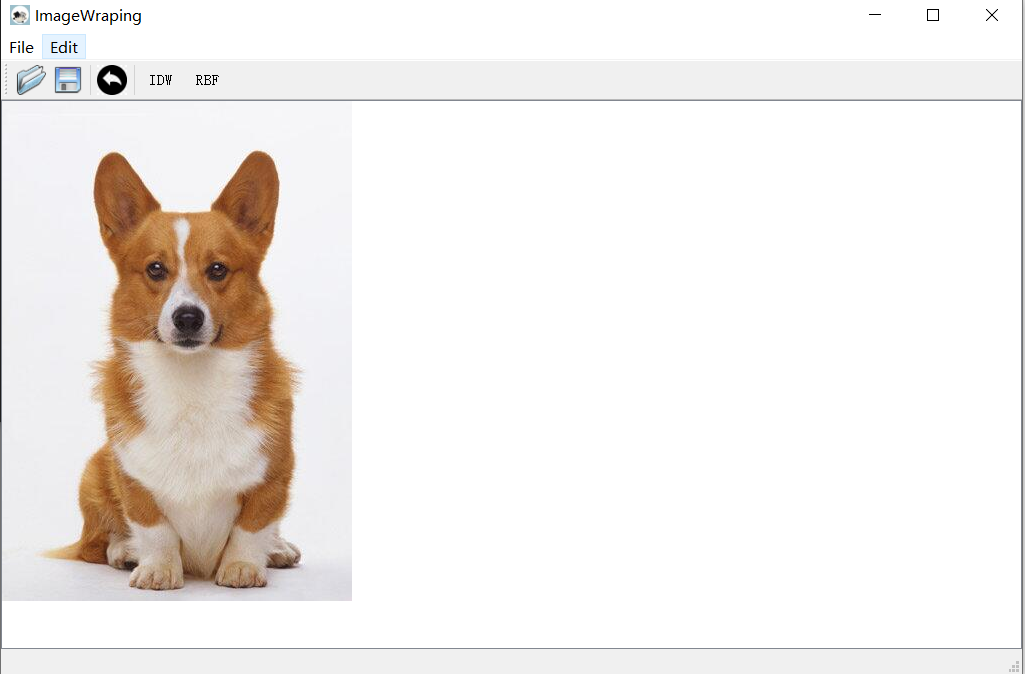
\includegraphics[width=3.3in]{./ui.png}
		\centering
		\caption{程序界面}
	\end{figure}
		
		\subsection{四边固定,四角内拉}

	\begin{figure}[H]
		\centering
		\subfigure[Action]{
			\begin{minipage}[t]{0.3\linewidth}
				\centering
				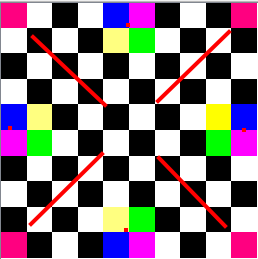
\includegraphics[width=1.6in]{./sample1.png}
				%\caption{fig1}
			\end{minipage}%
		}%
		\subfigure[IDW]{
			\begin{minipage}[t]{0.3\linewidth}
				\centering
				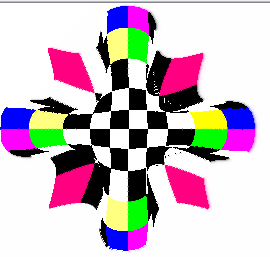
\includegraphics[width=1.7in]{./idw1.png}
				%\caption{fig2}
			\end{minipage}%
		}
		\subfigure[RBF]{
			\begin{minipage}[t]{0.3\linewidth}
				\centering
				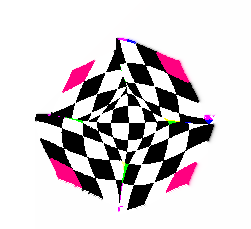
\includegraphics[width=1.7in]{./rbf1.png}
				%\caption{fig2}
			\end{minipage}%
		}
		\centering
		\caption{四边固定,四角内拉}
	\end{figure}
	
	\begin{figure}[H]
		\centering
		\subfigure[$\mu=0.5$]{
			\begin{minipage}[t]{0.3\linewidth}
				\centering
				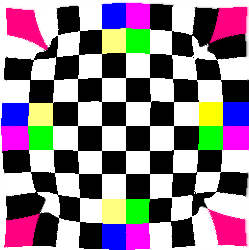
\includegraphics[width=1.6in]{./idw1u0.5.png}
				%\caption{fig1}
			\end{minipage}%
		}%
		\subfigure[$\mu=2$]{
			\begin{minipage}[t]{0.3\linewidth}
				\centering
				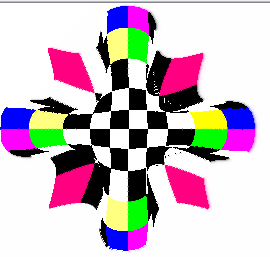
\includegraphics[width=1.7in]{./idw1.png}
				%\caption{fig2}
			\end{minipage}%
		}
		\subfigure[$\mu=4$]{
			\begin{minipage}[t]{0.3\linewidth}
				\centering
				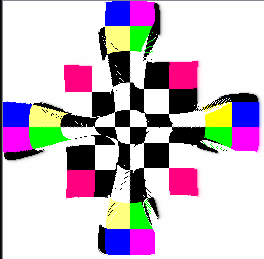
\includegraphics[width=1.7in]{./idw1u4.png}
				%\caption{fig2}
			\end{minipage}%
		}
		\centering
		\caption{IDW 不同$\mu$}
	\end{figure}
	
	\begin{figure}[H]
		\centering
		\subfigure[$\mu=-1$]{
			\begin{minipage}[t]{0.3\linewidth}
				\centering
				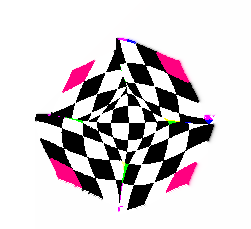
\includegraphics[width=1.8in]{./rbf1.png}
				%\caption{fig1}
			\end{minipage}%
		}%
		\subfigure[$\mu=-2$]{
			\begin{minipage}[t]{0.3\linewidth}
				\centering
				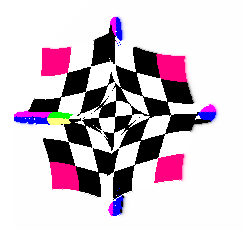
\includegraphics[width=1.7in]{./rbf1u2.png}
				%\caption{fig2}
			\end{minipage}%
		}
		\subfigure[$\mu=-10$]{
			\begin{minipage}[t]{0.3\linewidth}
				\centering
				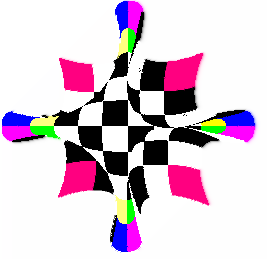
\includegraphics[width=1.7in]{./rbf1u10.png}
				%\caption{fig2}
			\end{minipage}%
		}
		\centering
		\caption{RBF 不同$\mu$}
	\end{figure}
	
	可以见到,在IDW算法中,$\mu$度量了给定配对点对其他点的影响力,当$\mu$越大,控制点能影响到的范围就越大;在RBF算法中同样如此。实验结果印证了理论分析。
	
	\subsection{四角固定,四边内拉}
	
	\begin{figure}[H]
		\centering
		\subfigure[Action]{
			\begin{minipage}[t]{0.3\linewidth}
				\centering
				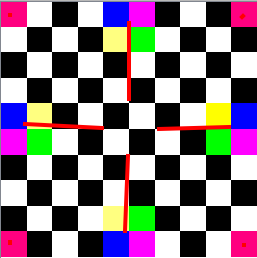
\includegraphics[width=1.6in]{./sample2.png}
				%\caption{fig1}
			\end{minipage}%
		}%
		\subfigure[IDW]{
			\begin{minipage}[t]{0.3\linewidth}
				\centering
				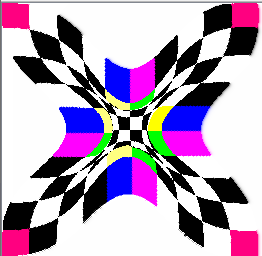
\includegraphics[width=1.7in]{./idw2.png}
				%\caption{fig2}
			\end{minipage}%
		}
		\subfigure[RBF]{
			\begin{minipage}[t]{0.3\linewidth}
				\centering
				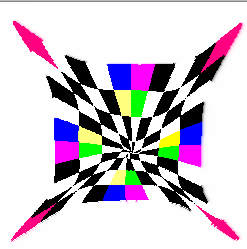
\includegraphics[width=1.7in]{./rbf2.png}
				%\caption{fig2}
			\end{minipage}%
		}
		\centering
		\caption{四角固定,四边内拉}
	\end{figure}
	
	\subsection{Interestings Images}
	
		\begin{figure}[H]
			\centering
			\subfigure[Action]{
				\begin{minipage}[t]{0.3\linewidth}
					\centering
					
\includegraphics[width=1.7in]{./m1.png}
					%\caption{fig1}
				\end{minipage}%
			}%
			\subfigure[source]{
				\begin{minipage}[t]{0.3\linewidth}
					\centering
					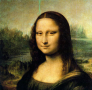
\includegraphics[width=1.7in]{./MonaLisa.png}
					%\caption{fig2}
				\end{minipage}%
			}
			\subfigure[result]{
				\begin{minipage}[t]{0.3\linewidth}
					\centering
					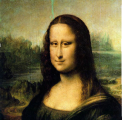
\includegraphics[width=1.7in]{./m1r.png}
					%\caption{fig2}
				\end{minipage}%
			}
			\centering
			\caption{Ex1.}
		\end{figure}
		
		\begin{figure}[H]
			\centering
			\subfigure[Action]{
				\begin{minipage}[t]{0.3\linewidth}
					\centering
					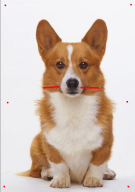
\includegraphics[width=1.3in]{./acdd.png}
					%\caption{fig1}
				\end{minipage}%
			}%
			\subfigure[source]{
				\begin{minipage}[t]{0.3\linewidth}
					\centering
					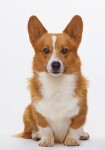
\includegraphics[width=1.3in]{./dd.png}
					%\caption{fig2}
				\end{minipage}%
			}
			\subfigure[result]{
				\begin{minipage}[t]{0.3\linewidth}
					\centering
					
\includegraphics[width=1.3in]{./fdd.png}
					%\caption{fig2}
				\end{minipage}%
			}
			\centering
			\caption{Ex2.}
		\end{figure}
	
	
	
	\section{实验总结}
	本次实验复现了图像变形的两种经典算法,直观验证了算法中参数对实际应用的作用,并学习了Qt的使用。
	
	附睿客网代码链接:https://rec.ustc.edu.cn/share/5a0b54b0-2f47-11ec-90e7-f14835723dfc
	
	\begin{thebibliography}{99}
	
		\bibitem{1}Image Warping Using few Anchor Points and Radial Functions:Nur Arad and Daniel Reisfeld.Computer Graphics Forum,1995.
		\bibitem{1}Image warping with scattered data interpolation:D. Ruprecht and H. Muller, IEEE Computer Graphics and Applications, vol. 15, no. 2, pp. 37-43, March 1995, doi: 10.1109/38.365004.
	\end{thebibliography}
\end{document}

